\documentclass[12pt]{article}
\usepackage{tikz}
\usepackage{geometry}

\usetikzlibrary{mindmap}

\author{ supercentinel }
%2019-01-01
\geometry{landscape, margin=1cm}

\begin{document}
\begin{center}
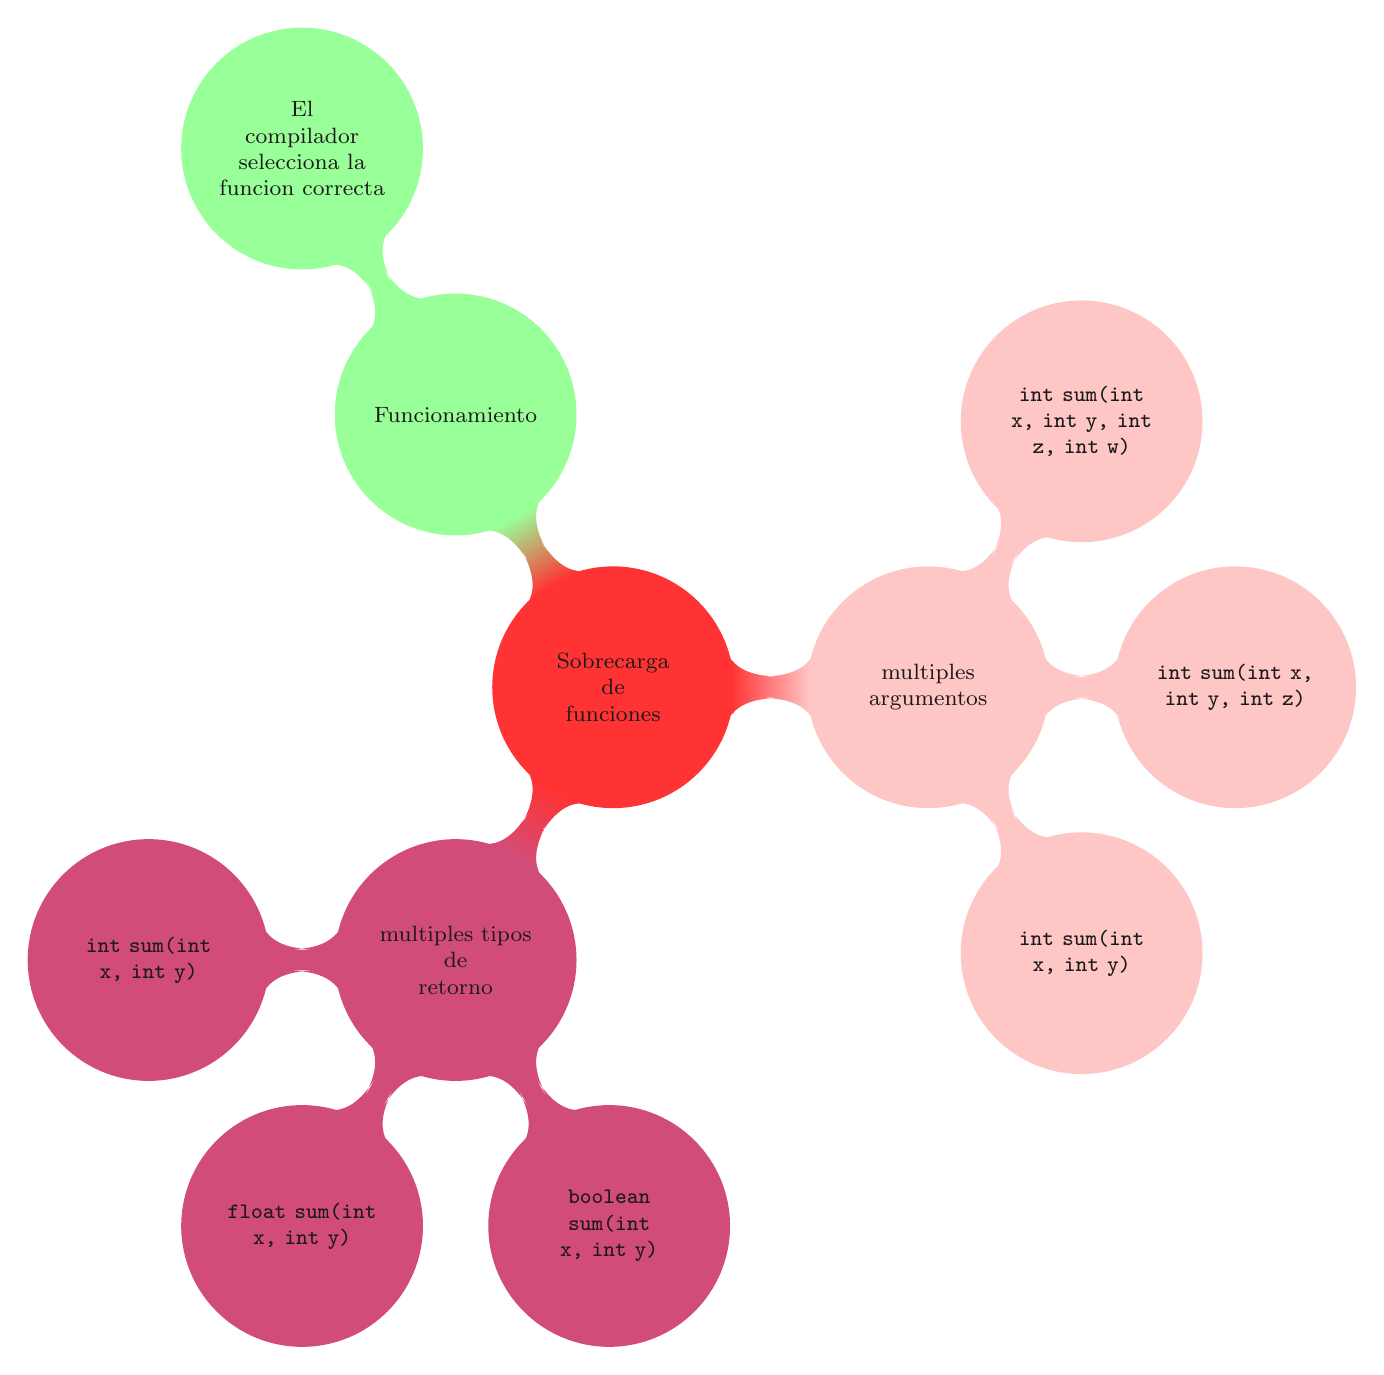
\begin{tikzpicture}[small mindmap, grow cyclic, every node/.style=concept, concept color=red!80, text=black!90, minimum size=3.0cm,
    level 1/.style={level distance=4.5cm,sibling angle=360/3},
    level 1/.style={level distance=4.0cm,sibling angle=360/3},
    level 2/.style={level distance=3.9cm,sibling angle=60},
    level 3/.style={level distance=3.5cm,sibling angle=60},
    ]
    \node{ Sobrecarga\\de\\funciones }
    child[concept color=purple!70] { node { multiples tipos\\de\\retorno }
        child { node { \texttt{int sum(int x, int y)} } }
        child { node { \texttt{float sum(int x, int y)} } }
        child { node { \texttt{boolean sum(int x, int y)} } }
    }
    child[concept color=pink!90] { node { multiples\\argumentos }
        child { node { \texttt{int sum(int x, int y)} } }
        child { node { \texttt{int sum(int x, int y, int z)} } }
        child { node { \texttt{int sum(int x, int y, int z, int w)} } }
    }
    child[concept color=green!40] { node { Funcionamiento }
        child { node { El\\compilador\\selecciona la\\funcion correcta } }
    }
    ;
\end{tikzpicture}
\end{center}
\end{document}
